\documentclass[a4paper]{report}
\usepackage{amsmath,amssymb,booktabs,bm,caption,enumerate,float,geometry,graphicx,indentfirst,setspace,titlesec}
\geometry{left=4.5cm,right=4.5cm,top=4cm,bottom=4cm}
\captionsetup[figure]{labelsep=period}
\captionsetup[table]{labelsep=period}
\begin{document}
	\renewcommand\thesection{\arabic{section}}
	\begin{Large}
		\begin{center}
			\setlength{\baselineskip}{14pt}
			\vspace{1.25cm}
			\rule[0cm]{11.2cm}{0.03em}\\
			\vspace{0.5cm}
			\textsc{UM-SJTU Joint Institute}\\
			\vspace{0.25cm}
			\textsc{Physics Laboratory\\(Vp141)}
			\vspace{0.3cm}
			\rule[0cm]{11.8cm}{0.05em}
			\vspace{4.9cm}\\
			\textsc{Laboratory Report}
		\end{center}
	\end{Large}
	\vspace{0.85cm}
	\begin{large}
		\begin{center}
			\textsc{Exercise 2}
			\\~
			\textsc{Measurement of Fluid Viscosity}
		\end{center}
		\vspace{6cm}
	\end{large}
	\begin{tabular}{l l l}
	Name: Yihua Liu&ID:518021910998&Group 9\\
	&&\\
	Date: 18 July 2019&&\\
	\end{tabular}
	\thispagestyle{empty}
	\newpage
	\section{Introduction}
	The Objective of the exercise is to experiment on the fluid viscosity that determines the fluid's flow. We can describe and measure the properties of some fluids with high viscosity by Stoke's method. For objects moving in a fluid, a drag force exerted on it in the opposite direction to its velocity is related to the shape, the speed, and the internal friction in the fluid quantified by the viscosity coefficient denoted as $\eta$.
	
	Considering the simplest situation -- a spherical object with the radius $R$ and its speed $v$ in an infinite volume of a liquid, the expression for the magnitude of the drag force is
	\begin{equation}
	F_1=6\pi\eta vR
	\end{equation}
	If it falls vertically downwards in a fluid, the viscous force $\bf{F}_1$ and the buoyancy force $\bf{F}_2$ upwards and the gravity $\bf{F}_3$ downwards, of which $\bf{F}_2$ is
	\begin{equation}
	F_2=\dfrac{4}{3}\pi R^3\rho_1 g
	\end{equation}
	and the weight of the object
	\begin{equation}
	F_3=mg=\dfrac{4}{3}\pi R^3\rho_2g
	\end{equation}
	where $rho_2$ is the density of the object. By balance equation, we have
	\begin{equation}
	\eta=\dfrac{2}{9}gR^2\dfrac{\rho_2-\rho_1}{v_t}=\dfrac{2}{9}gR^2\dfrac{(\rho_2-\rho_1)t}{s}=(3mg-4\rho_1\pi gR^3)\dfrac{s}{18\pi t}
	\end{equation}
	where the speed $v_t$ is a constant, $s$ is the distance that it traveled and $t$ the time from the origin until the object reaches terminal speed. Taking into consideration that finally the velocity of the motion is a constant, Eq. (4) has the following experimental form
	\begin{equation}
	\eta=\dfrac{mg-\dfrac{4}{3}\pi R^3\rho g}{6\pi v_tR(1+2.4\dfrac{R}{R_c})}=\dfrac{(mg-\dfrac{4}{3}\pi R^3\rho g)t}{6\pi sR(1+2.4\dfrac{R}{R_c})}
	\end{equation}
	where $R_c$ is the radius of an infinite long cylindral container.
	\section{Experimental setup}
	In this experiment, we use a set of Stoke's viscosity measurement device (see Figure 1) including conducting pipe, semiconductor laser generator, 3-D ajusting bracket, kerosene oil, and graduated flask. For measurement devices including micrometer, calliper, densimeter, electronic scales, stopwatch, and thermometer, we can measure various physical quantities of the motion of the small metal ball.
	\begin{figure}[H]
		\centering
		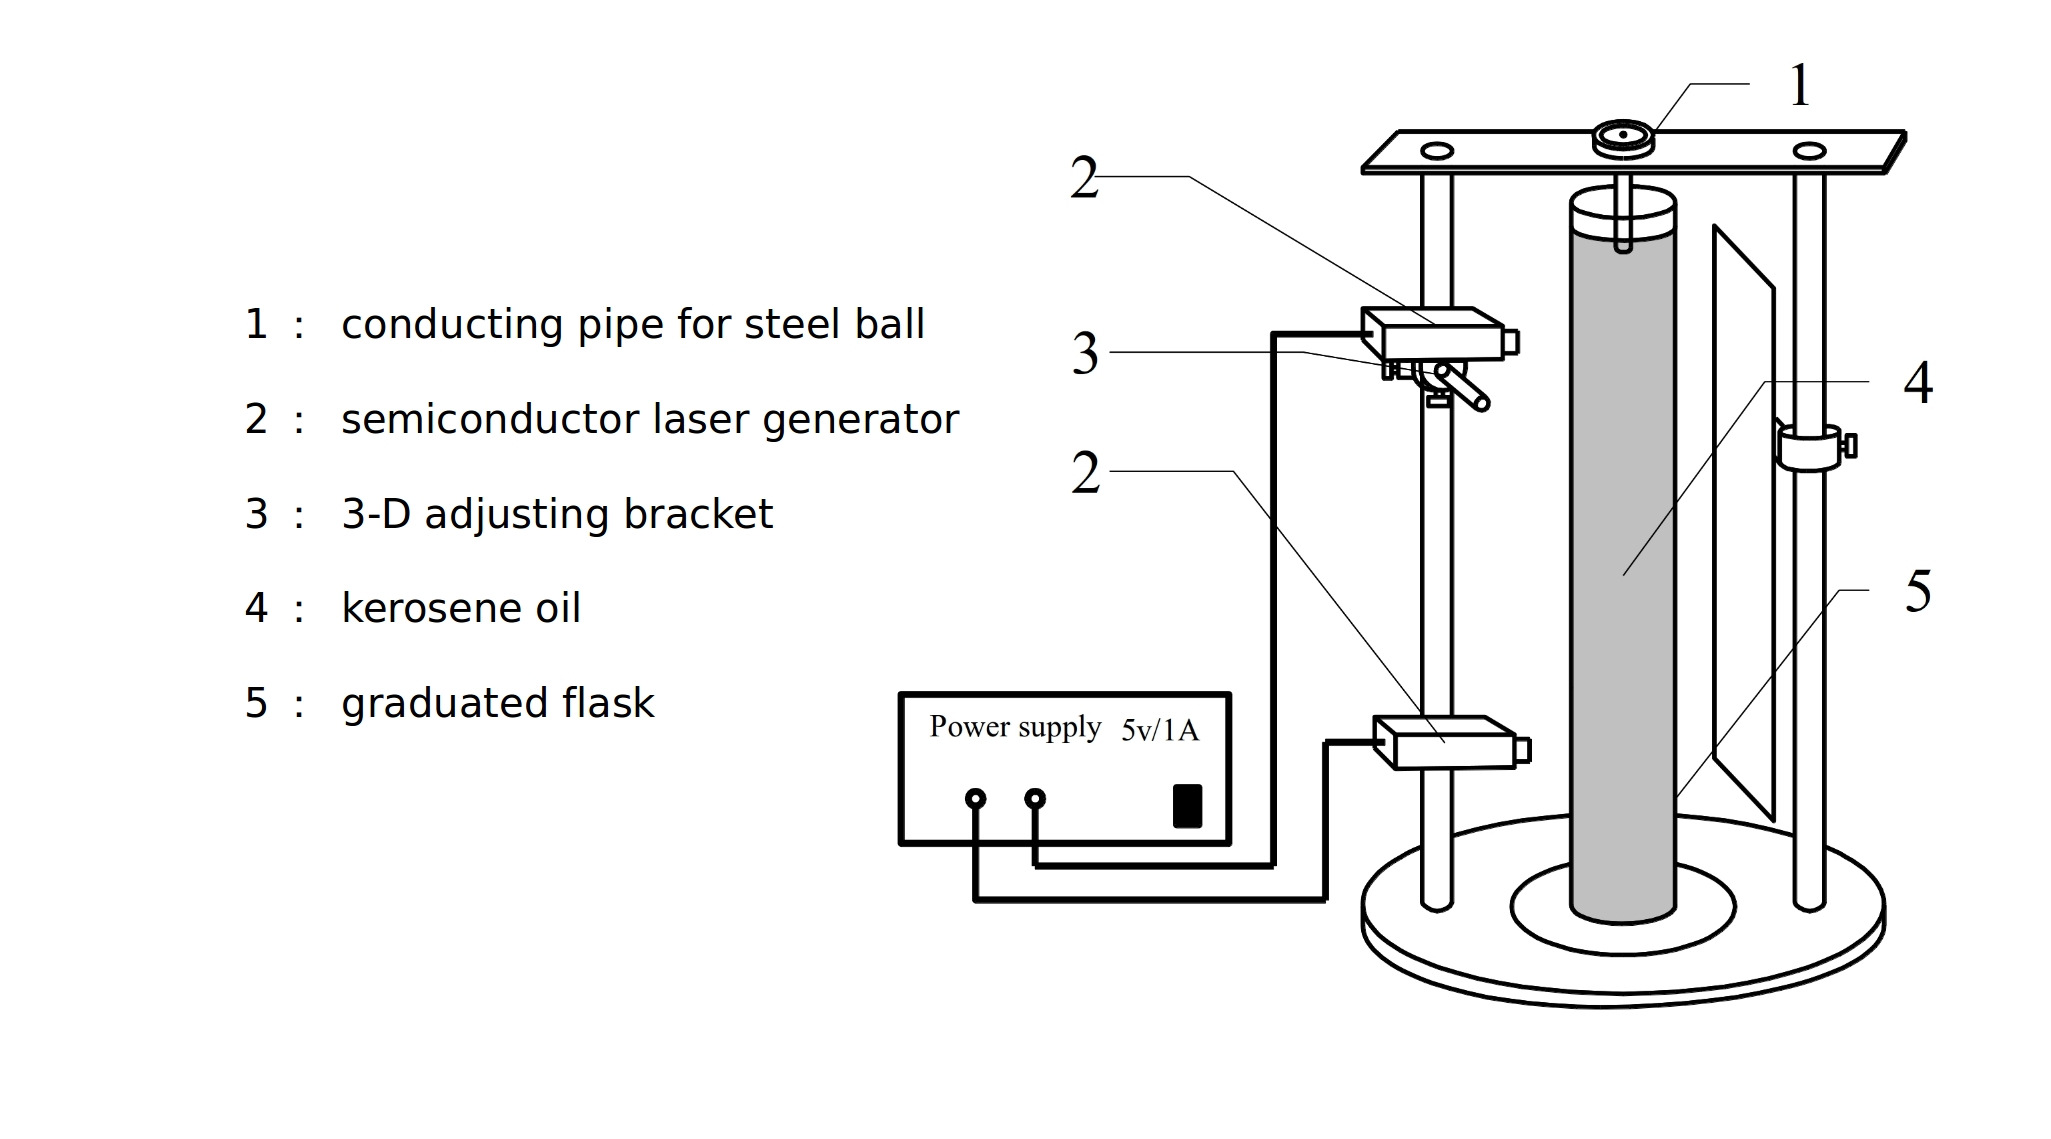
\includegraphics[width=1\linewidth]{1.jpg}
		\caption{Stokes' viscosity measurement apparatus.}
	\end{figure}
	To measure the positions of upper and lower laser beam, we use rule with maximum uncertainty $u=\pm 0.5$ mm. As the diameter of metal balls is very small, we use micrometer with maximum uncertainty $u=\pm 0.005$ mm. For stop watches, their undertainty $u=\pm 0.01$ s. The uncertainty of electronic scale used for measuring mass is $u=\pm 0.001$ g. Besides, we use the calliper with the uncertainty $u=\pm 0.02$ mm and the densimeter with $u=\pm 0.0005 \rm{g/{cm}^3}$.
	\section{Measurement}
	\subsection{Adjustment of the Stokes' viscosity measurement device}
	We first adjust the knobs beneath the base to ensure that the plumb aims just at center of the the base. Then we adjust the beams in order to make them parallel and aim at the plumb line by turning on the two lasers. After finishing adjustment, we remove the plumb and put the graduated flask together with castor oil at the center of the base. Finally, on the top of the Stokes' device we place the guilding pipe.
	\subsection{Measurement of the (constant) velocity of a falling ball}
	After the Stokes' device is settled, we measure the vertical distance $s$ between the two laser beams for three. Then we repeat doing this for three times. After the measurement, we prepare a metal ball in the guiding pipe and measure the time period $t$ with astopwatch when the ball passes through the first and the second beam for six times.
	\subsection{Measurement of constant quantities}
	In this experiment, to minimize errors, we measure the mass of the ball $m$ instead of the ball density $\rho_2$ just by electronic scales. To make the result more precise, we weight 40 metal balls and calculate the average mass of a single ball. Although we do not need to calculate the ball density, we are supposed to examine the diameter of the metal balls using micrometers for ten times. Then we calculate the average value as the diameter of the metal balls.
	\subsection{Calculation of the viscosity coefficient $\eta$}
	Using the formula Eq. (5), we calculate the value of viscosity coefficient $\eta$.
	\section{Results}
	\subsection{Distance}
	The distance between the two laser beams was measured in the procedure in section 3.2.
	\begin{equation*}
	\bar{x}_{A,1}=\dfrac{1}{3}\sum_{i=1}^{3}x_{A,i}=194.8\pm0.7\ \rm{mm}
	\end{equation*}
	and
	\begin{equation*}
	\bar{x}_{B,1}=\dfrac{1}{3}\sum_{i=1}^{3}x_{B,i}=60.2\pm0.7\ \rm{mm}
	\end{equation*}
	The distance traveled of the small metal ball is
	\begin{equation*}
	\bar{S}=\bar{x}_{A,1}-\bar{x}_{B,1}=134.7\pm0.7\ \rm{mm}
	\end{equation*}
	with the relative uncertainty 0.5\%.
	\begin{table}[H]
		\centering
		\begin{tabular}{|c|c|c|c|}
			\hline
			\multicolumn{4}{|c|}{distance $x$ [mm] $\pm$ 0.5 [mm]}\\
			\hline
			$x_{A,1}$&195.0&$x_{B,1}$&60.0\\
			\hline
			$x_{A,2}$&194.5&$x_{B,2}$&60.0\\
			\hline
			$x_{A,3}$&195.0&$x_{B,3}$&60.5\\
			\hline
		\end{tabular}
		\caption{Distance measurement data.}
	\end{table}
	\subsection{Time}
	The time that the small metal ball traveled from the first laser beam to the second was also measured in section 3.2.
	\begin{equation*}
	\bar{t}=\dfrac{1}{6}\sum_{i=1}^{6}t_i=6.60\pm0.03\ \rm{s}
	\end{equation*}
	with the relative uncertainty 0.5\%.
	\begin{table}[H]
		\centering
		\begin{tabular}{|c|c|c|c|}
			\hline
			\multicolumn{4}{|c|}{time $t$ [s] $\pm$ 0.01 [s]}\\
			\hline
			$t_1$&6.60&$t_4$&6.62\\
			\hline
			$t_2$&6.59&$t_5$&6.62\\
			\hline
			$t_3$&6.59&$t_6$&6.57\\
			\hline
		\end{tabular}
		\caption{Time measurement data.}
	\end{table}
	\subsection{Diameters of the Balls}
	The diameters of the balls was examined in section 3.3 with a micrometer.
	\begin{equation*}
	\bar{d}=\dfrac{1}{10}\sum_{i=1}^{10}t_i=1.992\pm0.006\ \rm{mm}
	\end{equation*}
	with the relative uncertainty 0.3\%.
	\begin{table}[H]
		\centering
		\begin{tabular}{|c|c|c|c|}
			\hline
			\multicolumn{4}{|c|}{diameter $d$ [mm] $\pm$ 0.005 [mm]}\\
			\hline
			$d_1$&1.995&$d_6$&1.990\\
			\hline
			$d_2$&1.990&$d_7$&1.990\\
			\hline
			$d_3$&1.990&$d_8$&2.000\\
			\hline
			$d_4$&1.990&$d_9$&1.990\\
			\hline
			$d_5$&1.995&$d_{10}$&1.990\\
			\hline
		\end{tabular}
		\caption{Measurement data for the diameters of the balls.}
	\end{table}
	\subsection{Inner Diameter of the Flask}
	The inner diameter of the flask was measured in section 3.3 with a calliper.
	\begin{equation*}
	\bar{D}=\dfrac{1}{6}\sum_{i=1}^{6}t_i=62.33\pm0.03\ \rm{mm}
	\end{equation*}
	with the relative uncertainty 0.05\%.
	\begin{table}[H]
		\centering
		\begin{tabular}{|c|c|c|c|}
			\hline
			\multicolumn{4}{|c|}{diameter $D$ [mm] $\pm$ 0.02 [mm]}\\
			\hline
			$D_1$&62.30&$D_4$&62.34\\
			\hline
			$D_2$&62.34&$D_5$&62.32\\
				\hline
			$D_3$&62.32&$D_6$&62.36\\
			\hline
		\end{tabular}
		\caption{Measurement data for the inner diameter of the flask.}
	\end{table}
	\subsection{Other Physcial Quantities}
	\begin{table}[H]
		\centering
		\begin{tabular}{|c|c|}
			\hline
			density of the castor oil $\rho_1$&$0.9570\ \left[\rm{g/{cm}^3}\right]\ \pm 0.0005\ \left[\rm{g/{cm}^3}\right]$\\
			\hline
			mass of 40 metal balls $m$&$1.312\ \left[\rm{g}\right]\ \pm 0.001\ \left[\rm{g}\right]$\\
			\hline
			temperature in the lab $T$&$25.4\ \left[\rm{^\circ C}\right]\ \pm 0.2\ \left[\rm{^\circ C}\right]$\\
			\hline
			acceleration due to gravity in the lab $g$&9.81 [$\rm{m/s^2}$]\\
			\hline
		\end{tabular}
	\caption{Values of other physical quantities.}
	\end{table}
	\subsection{Viscosity Coefficient}
	We first convert the quantities in the measurement to quantities in the formula Eq. (5). The mass of a single ball $m=\frac{1.312\ \rm{g}}{40}=0.0328\ \rm{g}=3.28\times10^{-5}\ \rm{kg}$. The radius of a metal ball is $R=\frac{d}{2}=0.996\ \rm{mm}=9.96\times10^{-4}\ \rm{m}$. The radius of the long cylindrical container is $R_c=\frac{D}{2}=31.165\ \rm{mm}=3.1165\times10^{-2}\ \rm{m}$. The density of the castor oil is $\rho=0.9570\ \rm{g/{cm}^3}=9.570\times10^2\ \rm{kg/m^3}$. The distance is $s=134.7\ \rm{mm}=0.1347\ \rm{m}$. The time is $t=6.60\ \rm{s}$.
	By Eq. (5), we can calculate the viscosity coefficient $\eta$ of the castor oil
	\begin{equation*}
	\eta=\dfrac{(m-\dfrac{4}{3}\pi R^3\rho)gt}{6\pi sR(1+2.4\dfrac{R}{R_c})}=0.686\ \rm{Pa\cdot s}
	\end{equation*}
	\section{Conclusions and discussion}
	In this experiment, we use Stokes' method to measure the viscosity coefficient of castor oil. However, there are some corrections. For example, to minimize type-B uncertainties, we use the mass of the ball instead of the ball density to calculate the viscosity coefficient. Besides, the final uncertainty turns out to be great because of some possible erros when measuring the diamter of one single metal ball. When using a micrometer, it is important not to compress the ball but also keep it contact compactly.
	
	On the other hand, there are probably some remaining castor oil on the surface of the metal balls so that when measuring the mass of 40 metal balls the result might be greater than expected.
	
	Besides, when applying the formula Eq. (5), it is actually a simulation based on experiments rather than theories, since the cylindrical container cannot have infinite length.
	
	To improve this experiment, I think carefully cleaning the ball can reduce errors when measuring the mass of 40 metal balls.
	\newpage
	\renewcommand\thesection{\Alph{section}}
	\setcounter{section}{0}
	\section{Measurement uncertainty analysis}
	\subsection{Uncertainty of distance measurements}
	\begin{equation*}
	\sigma_{x_A}=\sqrt{\dfrac{\sum_{i=1}^3(\bar{x}_A-x_{A,i})^2}{3-1}}=0.289\ \rm{mm}
	\end{equation*}
	\begin{equation*}
	\Delta_A=\dfrac{t_{0.95}}{\sqrt{3}}\sigma_{x_A}=0.534\ \rm{mm}
	\end{equation*}
	\begin{equation*}
	\Delta_B=0.5\ \rm{mm}
	\end{equation*}
	\begin{equation*}
	u_{x_A}=\sqrt{\Delta_A^2+\Delta_B^2}=0.7\ \rm{mm}
	\end{equation*}
	\begin{equation*}
	\sigma_{x_B}=\sqrt{\dfrac{\sum_{i=1}^3(\bar{x}_B-x_{B,i})^2}{3-1}}=0.289\ \rm{mm}
	\end{equation*}
	\begin{equation*}
	\sigma_{x_A}=\sigma_{x_B}
	\end{equation*}
	\begin{equation*}
	u_{x_B}=u_{x_A}=\sqrt{\Delta_A^2+\Delta_B^2}=0.7\ \rm{mm}
	\end{equation*}
	\begin{equation*}
	u_s=0.7\ \rm{mm}
	\end{equation*}
	\begin{equation*}
	u_{rs}=\dfrac{u_s}{s}\times100\%=0.5\%
	\end{equation*}
	\begin{equation*}
	s=134.7\pm0.7\ \rm{mm}
	\end{equation*}
	\subsection{Uncertainty of time measurements}
	\begin{equation*}
	\sigma_t=\sqrt{\dfrac{\sum_{i=1}^6(\bar{t}-t_i)^2}{6-1}}=0.0194\ \rm{s}
	\end{equation*}
	\begin{equation*}
	\Delta_A=\dfrac{t_{0.95}}{\sqrt{6}}\sigma_t=0.0254\ \rm{s}
	\end{equation*}
	\begin{equation*}
	\Delta_B=0.01\ \rm{mm}
	\end{equation*}
	\begin{equation*}
	u_t=\sqrt{\Delta_A^2+\Delta_B^2}=0.03\ \rm{s}
	\end{equation*}
	\begin{equation*}
	u_{rt}=\dfrac{u_t}{t}\times100\%=0.5\%
	\end{equation*}
	\begin{equation*}
	t=6.60\pm0.03\ \rm{s}
	\end{equation*}
	\subsection{Uncertainty of measurements for the diameters of the balls}
	\begin{equation*}
	\sigma_d=\sqrt{\dfrac{\sum_{i=1}^{10}(\bar{t}-t_i)^2}{10-1}}=0.00350\ \rm{mm}
	\end{equation*}
	\begin{equation*}
	\Delta_A=\dfrac{t_{0.95}}{\sqrt{10}}\sigma_d=0.00354\ \rm{mm}
	\end{equation*}
	\begin{equation*}
	\Delta_B=0.005\ \rm{mm}
	\end{equation*}
	\begin{equation*}
	u_d=\sqrt{\Delta_A^2+\Delta_B^2}=0.006\ \rm{mm}
	\end{equation*}
	\begin{equation*}
	u_{rd}=\dfrac{u_d}{d}\times100\%=0.3\%
	\end{equation*}
	\begin{equation*}
	d=1.992\pm0.006\ \rm{mm}
	\end{equation*}
	\subsection{Uncertainty of measurements for the inner diameter of the flask}
	\begin{equation*}
	\sigma_D=\sqrt{\dfrac{\sum_{i=1}^{6}(\bar{t}-t_i)^2}{6-1}}=0.0210\ \rm{mm}
	\end{equation*}
	\begin{equation*}
	\Delta_A=\dfrac{t_{0.95}}{\sqrt{6}}\sigma_D=0.0274\ \rm{mm}
	\end{equation*}
	\begin{equation*}
	\Delta_B=0.02\ \rm{mm}
	\end{equation*}
	\begin{equation*}
	u_D=\sqrt{\Delta_A^2+\Delta_B^2}=0.03\ \rm{mm}
	\end{equation*}
	\begin{equation*}
	u_{rD}=\dfrac{u_D}{D}\times100\%=0.05\%
	\end{equation*}
	\begin{equation*}
	D=62.33\pm0.03\ \rm{mm}
	\end{equation*}
	\subsection{Uncertainty of measurements for the mass of one ball}
	\begin{equation*}
	u_m=\dfrac{0.001\ \rm{g}}{40}=2.5\times10^{-5}\ \rm{g}
	\end{equation*}
	\begin{equation*}
	m=(3.28\pm0.0025)\times10^{-5}\ \rm{kg}
	\end{equation*}
	\subsection{Uncertainty of measurements for the density of the castor oil}
	Since the measurements of the density of the castor oil were single measurements with type-B uncertainty of 0.0005 $\rm{g/{cm}^3}$, the uncertainty is $u_{\rho}=0.0005\ \rm{g/{cm}^3}$.
	\subsection{Uncertainty of the viscosity coefficient}
	Substitute $D$ for $R_c$ and $d$ for $R$ and denote the density of the castor oil as $\rho_1$, we have the expression of the viscosity
	\begin{equation*}
	\eta=\dfrac{g}{18}(\dfrac{6m}{\pi d}-\rho_1d^2)\dfrac{t}{s}\dfrac{D}{D+2.4d}
	\end{equation*}
	The uncertainty of the viscosity coefficient $\eta$ can be calculated as
	\begin{equation*}
	u_{\eta}=\sqrt{(\dfrac{\partial\eta}{\partial d}u_d)^2+(\dfrac{\partial\eta}{\partial D}u_D)^2+(\dfrac{\partial\eta}{\partial s}u_s)^2+(\dfrac{\partial\eta}{\partial t}u_t)^2+(\dfrac{\partial\eta}{\partial\rho_1}u_{\rho_1})^2+(\dfrac{\partial\eta}{\partial m}u_m)^2}
	\end{equation*}
	Calculating the six partical derivatives respectively,
	\begin{equation*}
	\dfrac{\partial\eta}{\partial d}=-\dfrac{gD}{18}(\dfrac{6m}{\pi}\dfrac{D+4.8d}{d^2(D+2.4d)^2}+\rho_1\dfrac{2Dd+2.4d^2}{(D+2.4d)^2})\dfrac{t}{s}
	\end{equation*}
	\begin{equation*}
	\dfrac{\partial\eta}{\partial D}=\dfrac{g}{18}(\dfrac{6m}{\pi d}-\rho_1d^2)\dfrac{t}{s}\cdot\dfrac{2.4d}{(D+2.4d)^2}
	\end{equation*}
	\begin{equation*}
	\dfrac{\partial\eta}{\partial s}=-\dfrac{g}{18}(\dfrac{6m}{\pi d}-\rho_1d^2)\dfrac{t}{s^2}\cdot\dfrac{D}{D+2.4d}
	\end{equation*}
	\begin{equation*}
	\dfrac{\partial\eta}{\partial t}=\dfrac{g}{18}(\dfrac{6m}{\pi d}-\rho_1d^2)\dfrac{1}{s}\cdot\dfrac{D}{D+2.4d}
	\end{equation*}
	\begin{equation*}
	\dfrac{\partial\eta}{\partial\rho_1}=-\dfrac{g}{18}\dfrac{td^2}{s}\cdot\dfrac{D}{D+2.4d}
	\end{equation*}
	\begin{equation*}
	\dfrac{\partial\eta}{\partial m}=\dfrac{g}{18}(\dfrac{6}{\pi d})\dfrac{t}{s}\cdot\dfrac{D}{D+2.4d}
	\end{equation*}
	We have the uncertainty of the viscosity coefficient
	\begin{equation*}
	u_{\eta}=\sqrt{(\dfrac{\partial\eta}{\partial d}u_d)^2+(\dfrac{\partial\eta}{\partial D}u_D)^2+(\dfrac{\partial\eta}{\partial s}u_s)^2+(\dfrac{\partial\eta}{\partial t}u_t)^2+(\dfrac{\partial\eta}{\partial\rho_1}u_{\rho_1})^2+(\dfrac{\partial\eta}{\partial m}u_m)^2}=0.6\ \rm{Pa\cdot s}
	\end{equation*}
	with the relative uncertainty
	\begin{equation*}
	u_{r\eta}=\dfrac{u_{\eta}}{\eta}\times100\%=87\%.
	\end{equation*}
	\section{Data Sheet}
	\begin{figure}[H]
		\centering
		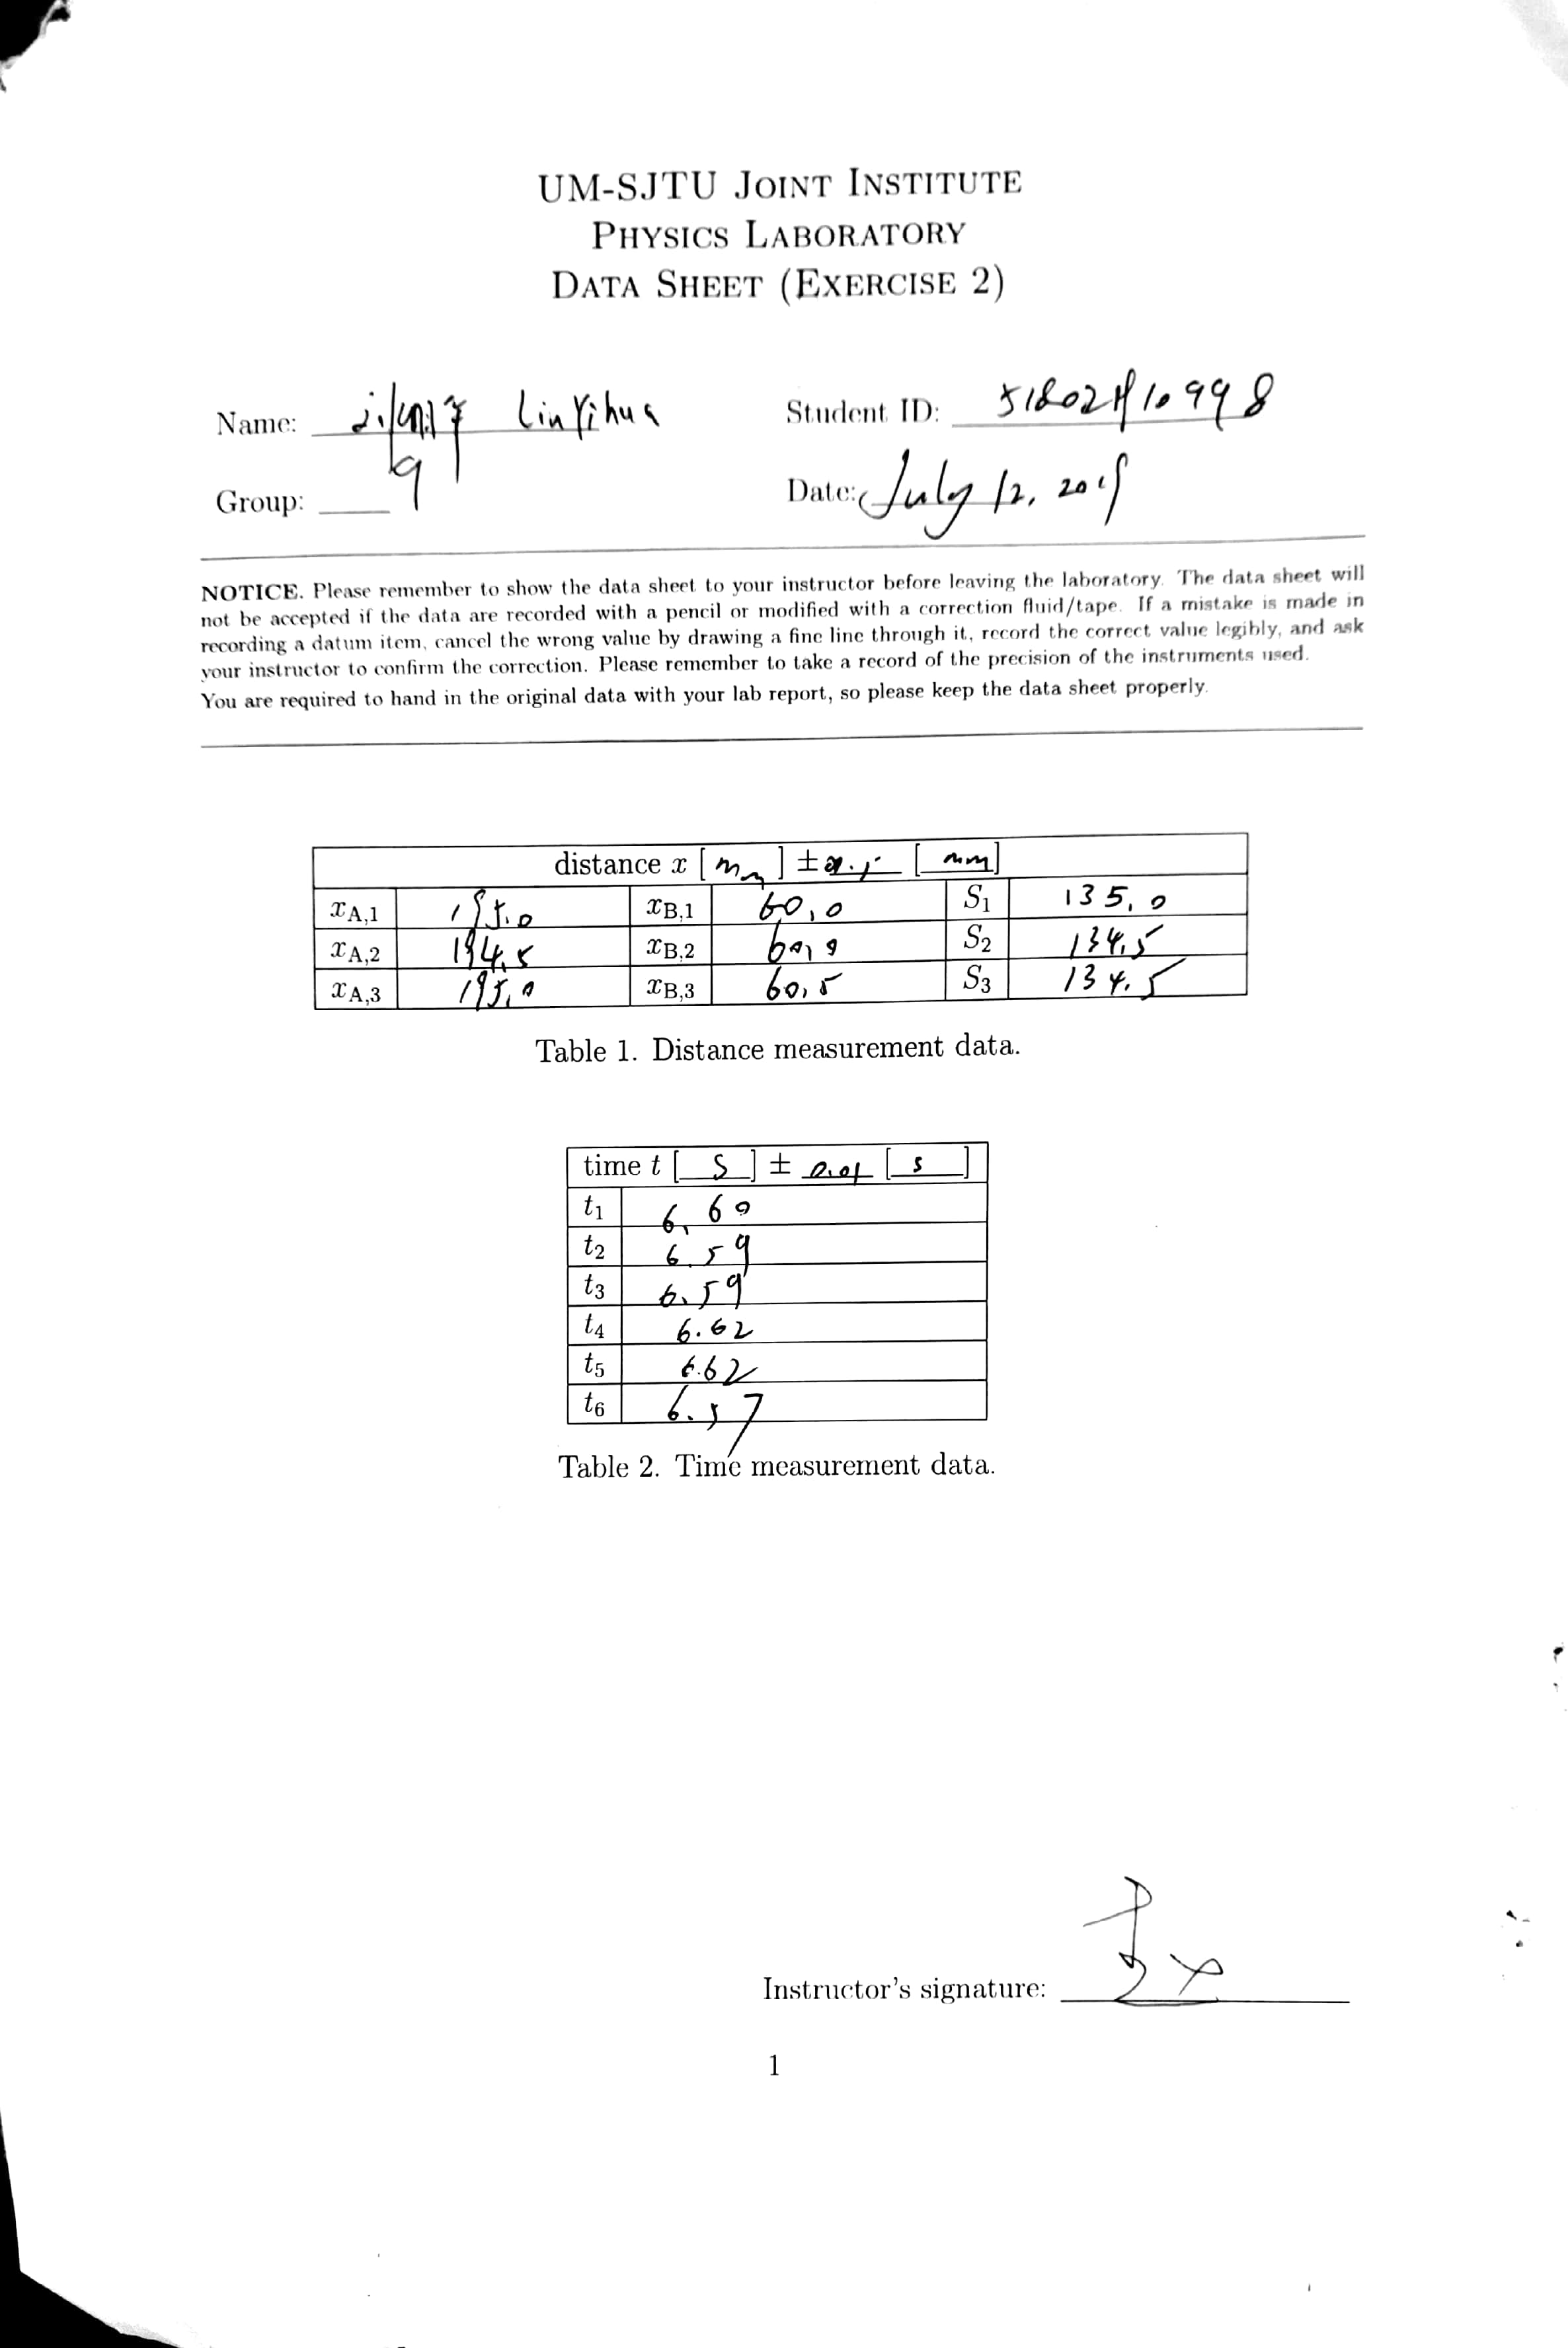
\includegraphics[width=1\linewidth]{2.jpg}
	\end{figure}
	\begin{figure}[H]
		\centering
		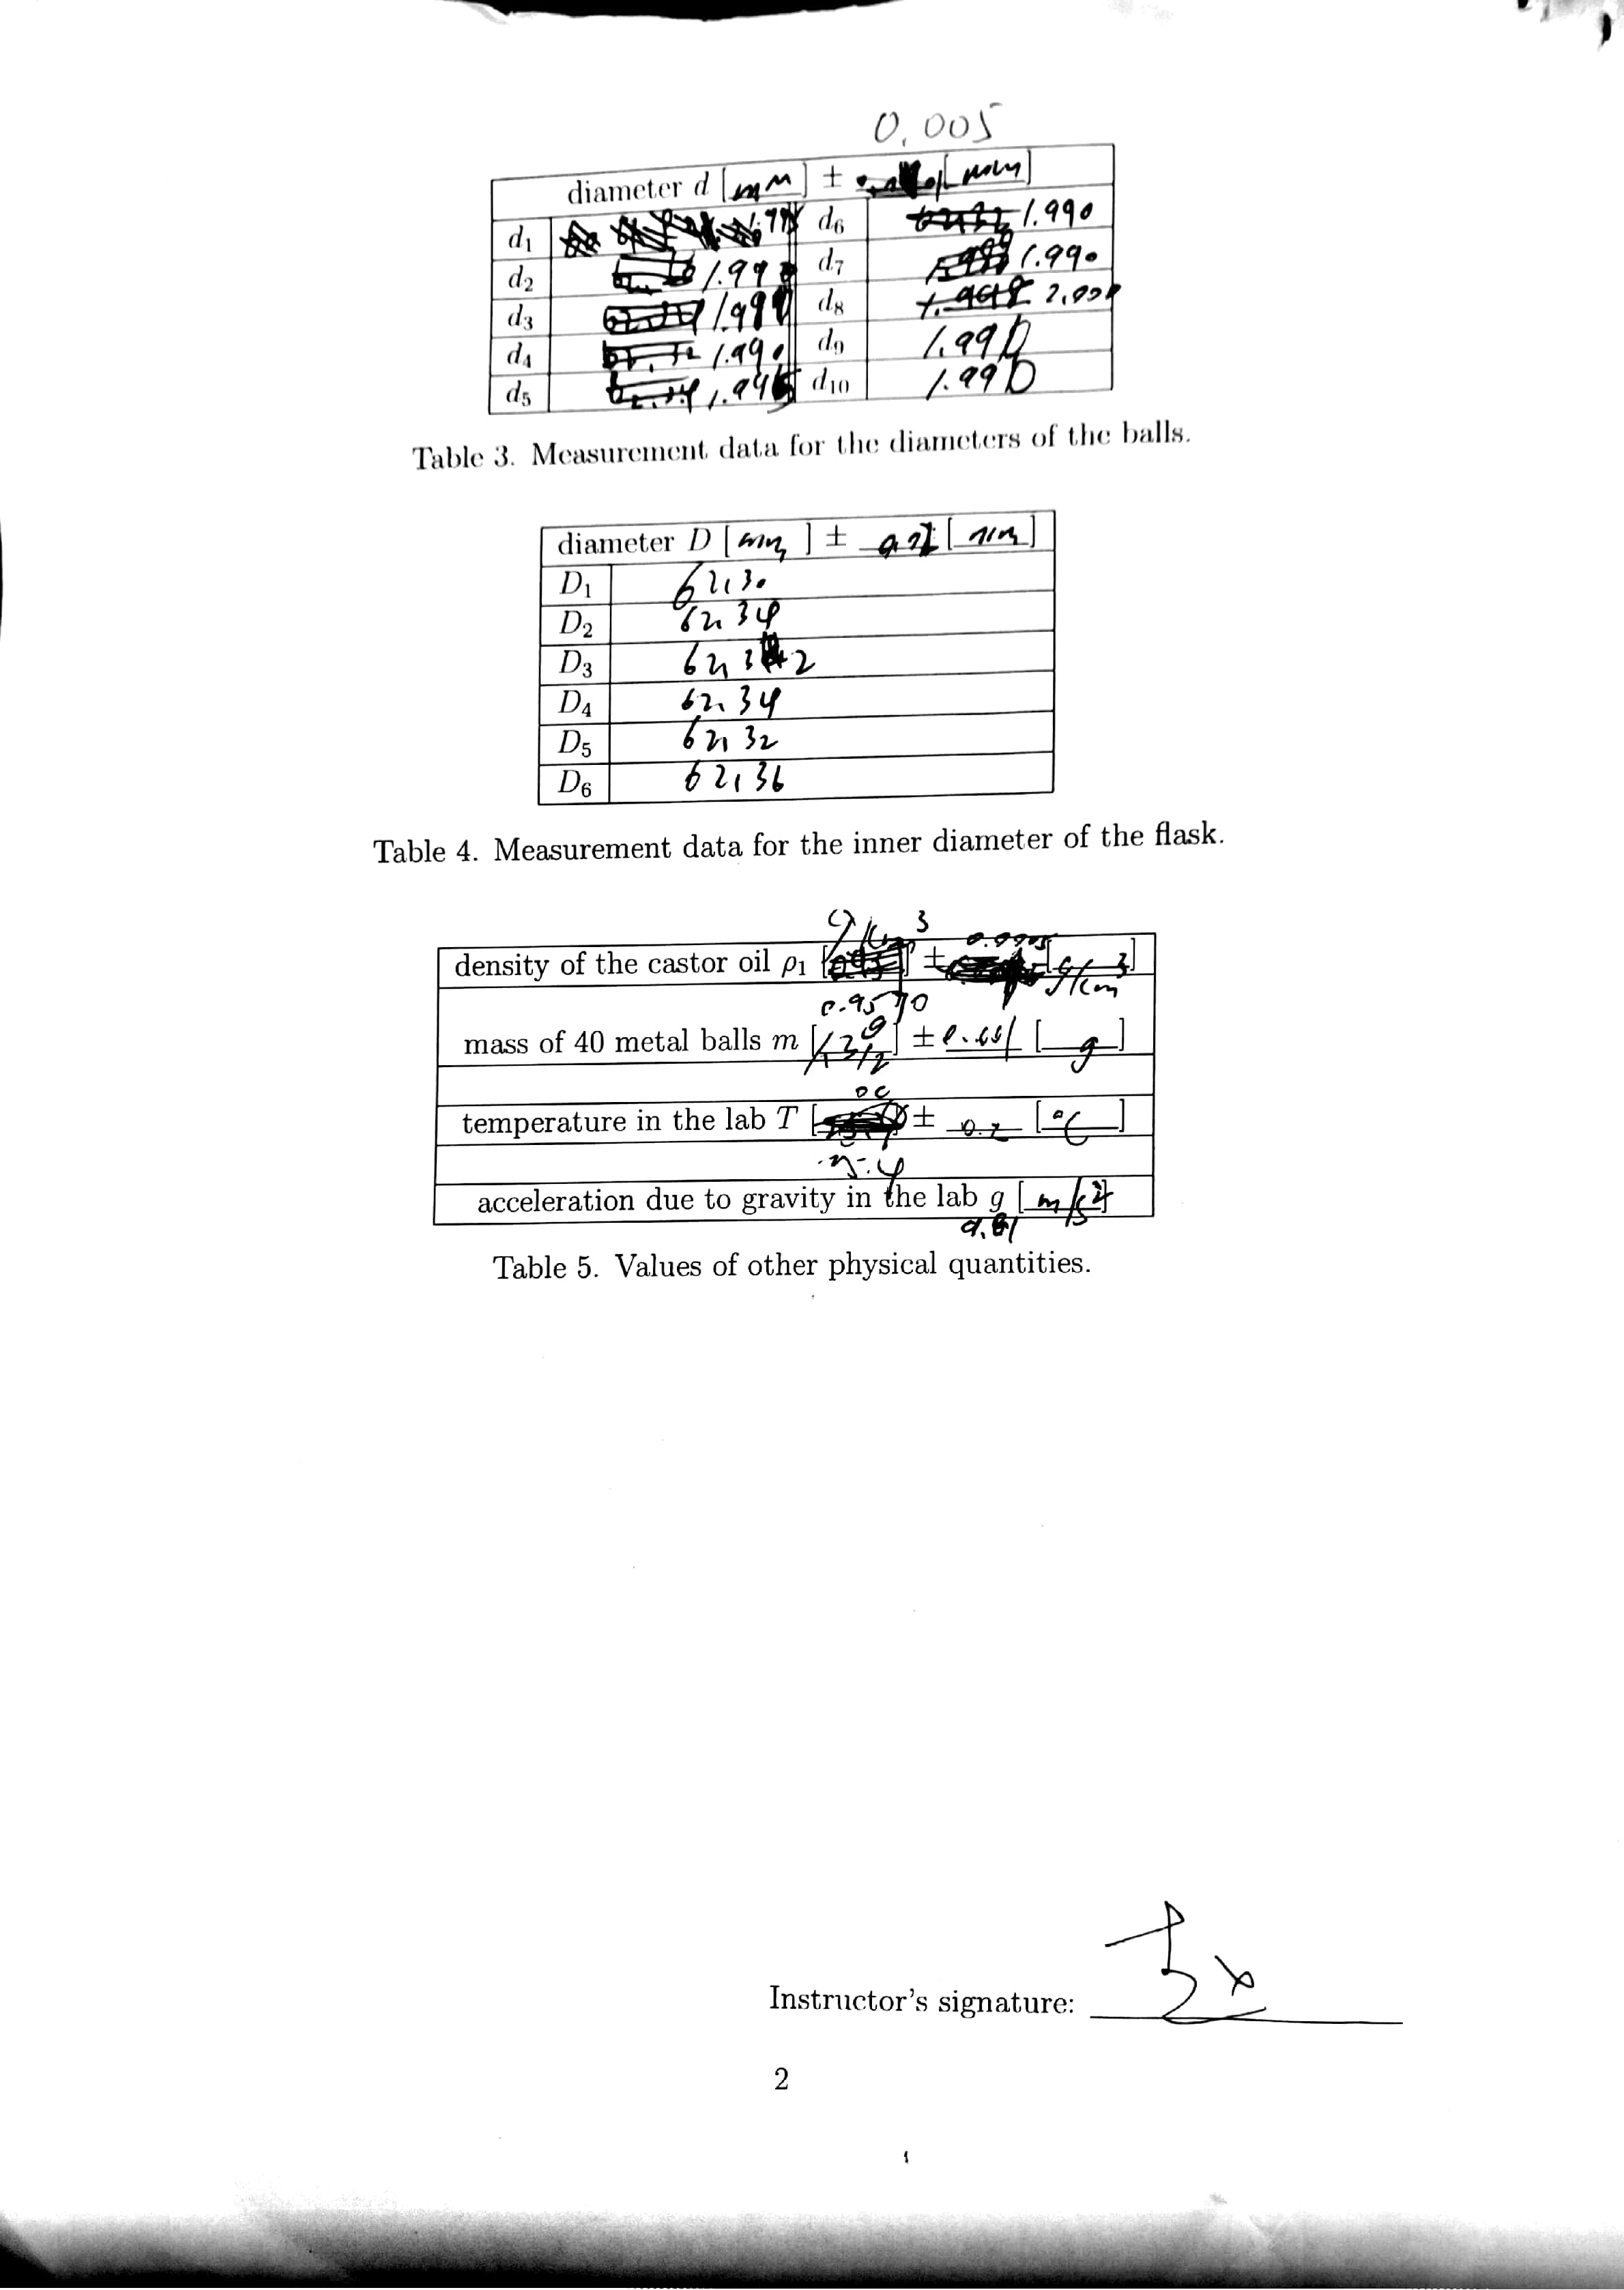
\includegraphics[width=1\linewidth]{3.jpg}
	\end{figure}
\end{document}